\documentclass[tikz,border=6pt]{standalone}
\usepackage{tikz}\usetikzlibrary{arrows.meta}
\definecolor{nebula}{HTML}{6366F1}\definecolor{spark}{HTML}{14B8A6}\definecolor{ink}{HTML}{334155}
\begin{document}
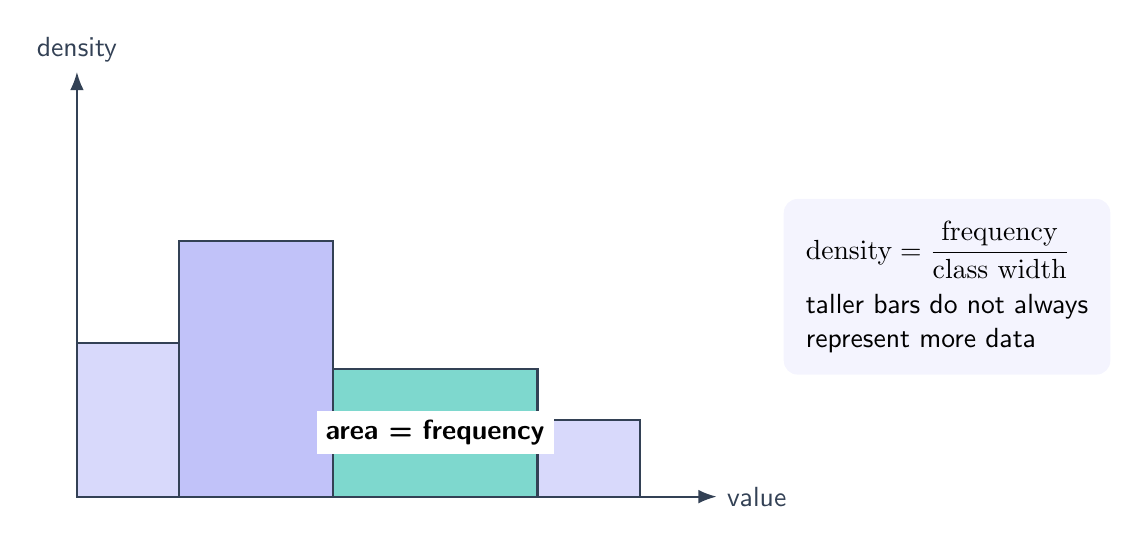
\begin{tikzpicture}[font=\sffamily,>=Latex,x=0.65cm,y=0.65cm]
  \draw[->,thick,ink] (0,0)--(12.5,0) node[right] {value}; \draw[->,thick,ink] (0,0)--(0,8.3) node[above] {density};
  \fill[nebula!25] (0,0) rectangle (2,3); \fill[nebula!40] (2,0) rectangle (5,5); \fill[spark!55] (5,0) rectangle (9,2.5); \fill[nebula!25] (9,0) rectangle (11,1.5);
  \draw[thick,ink] (0,0) rectangle (2,3); \draw[thick,ink] (2,0) rectangle (5,5); \draw[thick,ink] (5,0) rectangle (9,2.5); \draw[thick,ink] (9,0) rectangle (11,1.5);
  \node[fill=white] at (7,1.25) {\bfseries area = frequency};
  \node[align=left,fill=nebula!7,rounded corners=5pt,inner sep=8pt] at (17,4.1) {$\displaystyle \mathrm{density}=\frac{\mathrm{frequency}}{\mathrm{class\ width}}$\\[5pt]taller bars do not always\\represent more data};
\end{tikzpicture}
\end{document}
